Photolithography in the context of micro- and nano-technology it is a \emph{selection} processes where instead of adding or removing material of the wafer (like in deposition or ethcing) we are selecting which regions of the wafer to be exposed to the subsequent steps.

It originates from the words Photo (with light) and Lithography, from the Greek \textit{lithos} (stone) and \textit{graphein} (to write). Where instead of using stone and ink we use light in order to transfer the logic of a certain geometry into our silicon wafer.

Photolithography became fundemental due to batch fabrication where growing/depositing or etching films only in certain areas (selectively) is hard and expensive. To simplify the process, these selective patterns are created once (on a mask) and then we can transfer these patterns to as many wafers as needed using light.

\subsubsection*{Principle of photolithography}

The purpose of photolithography is to transfer a desired two-dimensional pattern from a master copy (the \emph{mask}) into a photosensitive polymer layer called the \emph{photoresist}, coated onto the wafer surface. After pattern transfer the patterned resist acts as a stencil, protecting or exposing specific areas during etching, deposition, or ion implantation \cite{FundTechProc2024}.

A photomask is a high-purity, amorphous SiO$_2$ (quartz) slab on which an absorbing chromium layer has been patterned by laser or electron-beam lithography. Quartz is chosen because it maintains high optical transmission even at ultraviolet wavelengths (below 300\,nm) where soda-lime glass becomes opaque, as shown in Figure~\ref{fig:mask_transmission} \cite{MitaniMicroMask}.

\begin{figure}[htbp]
  \centering
  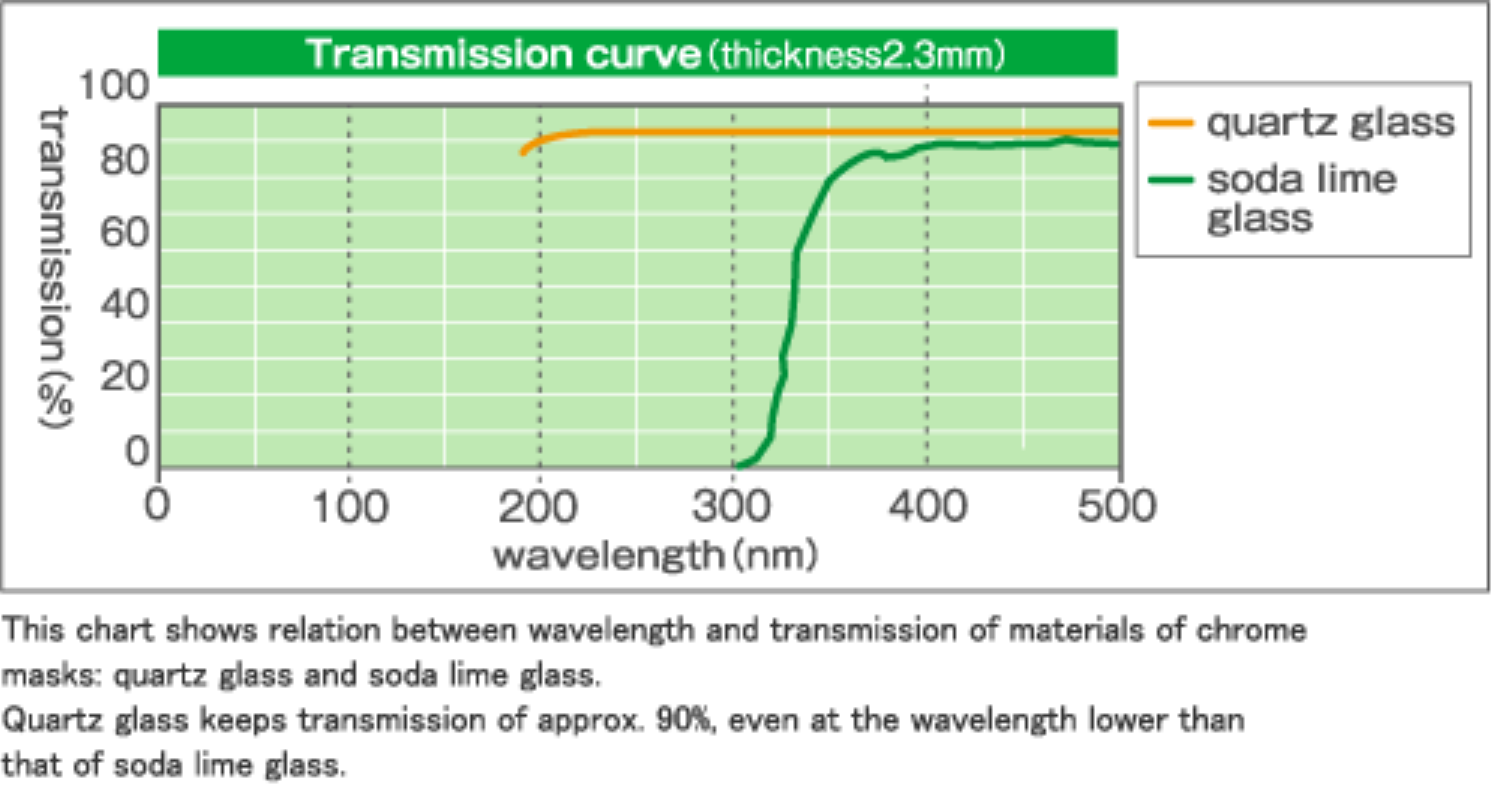
\includegraphics[width=0.6\textwidth]{piquet/images/mask_transmission.png}
  \caption{Transmission curves for quartz glass and soda-lime glass as a function of wavelength.
           Quartz maintains $\sim$90\,\% transmission down to wavelengths below 200\,nm, whereas
           soda-lime glass cuts off around 300\,nm, making quartz the required substrate for
           UV photomasks \cite{MitaniMicroMask}.}
  \label{fig:mask_transmission}
\end{figure} 

Because a single device requires many sequential patterning steps, precise alignment of each new mask to the previously printed features on the wafer is critical; misalignment can arise from X--Y displacement or rotational error, and is corrected by superimposing dedicated alignment marks using a split-field microscope.

\subsubsection*{Photoresists}

A photoresist is a photosensitive organic mixture composed of three main constituents:
      
(i) an inactive \emph{polymer resin} that provides mechanical rigidity, adhesion and chemical resistance.

(ii) a \emph{PhotoActive Compound} (PAC) responsible for the photosensitive response.

(iii) a \emph{solvent} that keeps the mixture liquid for spin-coating and controls film thickness through its viscosity.

Photoresists are classified by their \emph{polarity}:

\begin{itemize}
    \item \textbf{Positive resists.} Exposure to photons breaks polymer chains (chain scission), rendering the exposed areas more soluble in the developer solution. After development, windows open where the mask was transparent, replicating the mask pattern directly.
    \item \textbf{Negative resists.} Exposure induces cross-linking of the polymer chains, making the illuminated regions \emph{less} soluble. After development, the unexposed areas are dissolved and the exposed areas remain, producing the inverse (negative-tone) of the mask.
\end{itemize}

\begin{figure}[htbp]
  \centering
  \begin{minipage}[t]{0.46\textwidth}
    \centering
    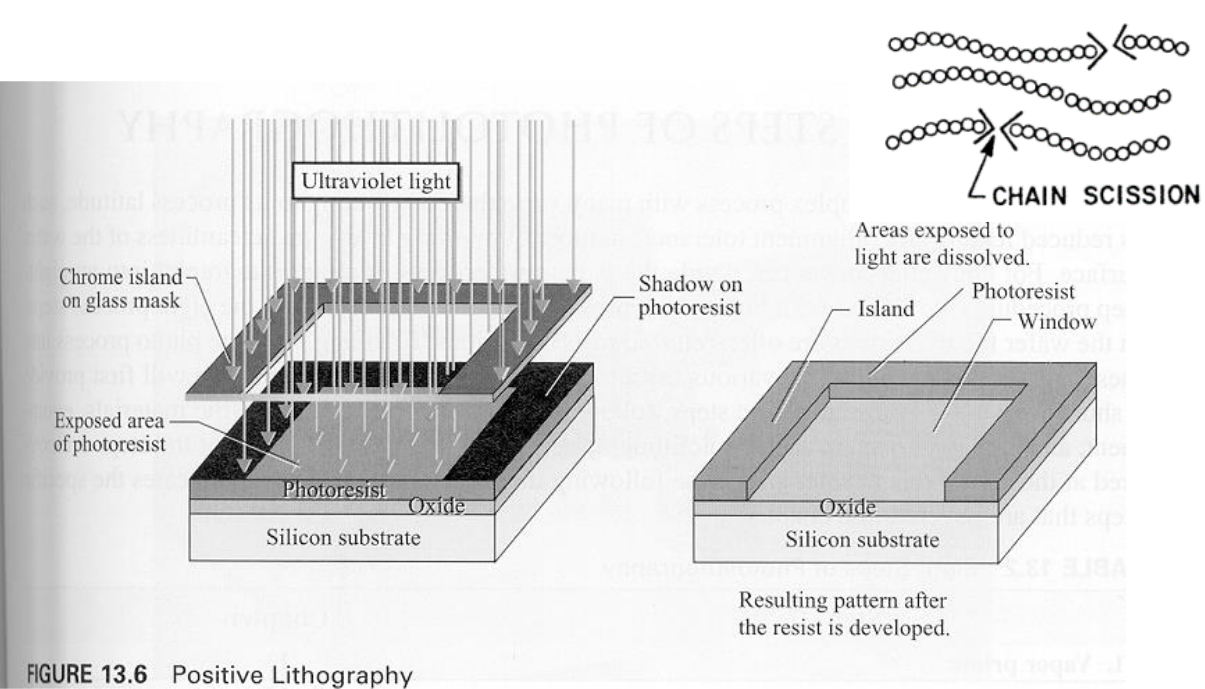
\includegraphics[width=\textwidth]{piquet/images/pos_lithography.png}
    \label{fig:pos_resist}
  \end{minipage}
  \hfill
  \begin{minipage}[t]{0.46\textwidth}
    \centering
    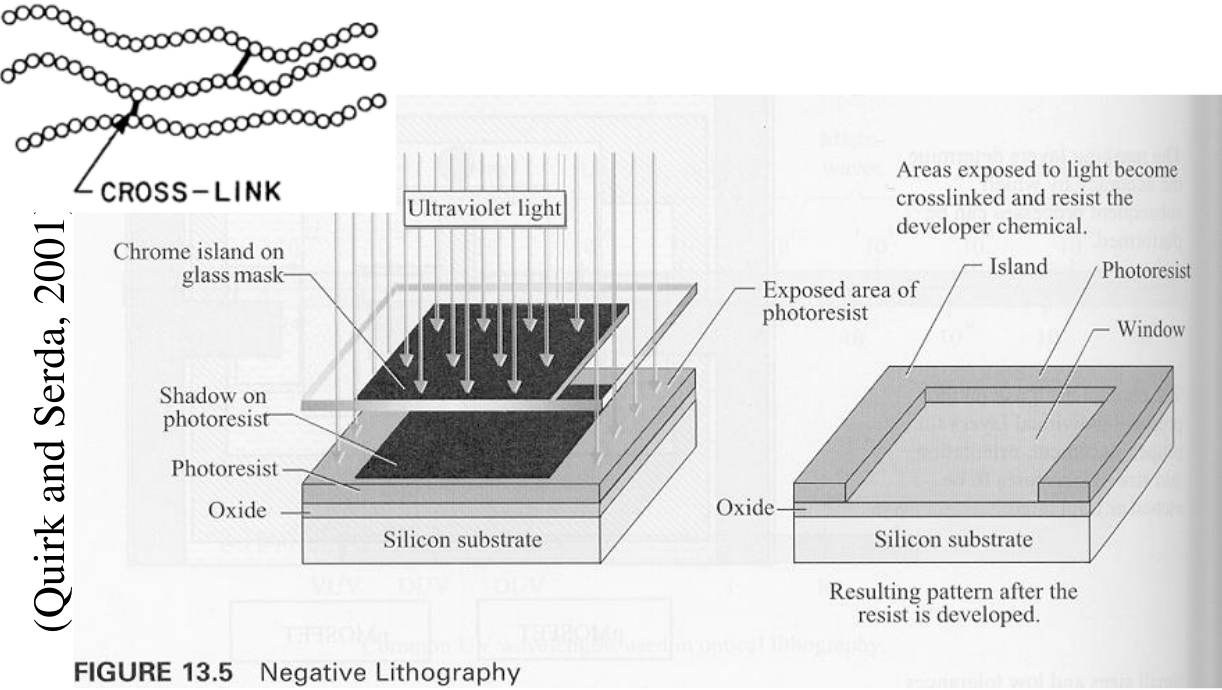
\includegraphics[width=\textwidth]{piquet/images/neg_lithography.png}
    \label{fig:neg_resist}
  \end{minipage}
  \caption{Comparison of positive and negative photoresist behaviour after UV exposure and development \cite{FundTechProc2024}.}
  \label{fig:pos_neg_resist}
\end{figure}

Positive resists generally offer better resolution because the chain-scission fragments are smaller than the cross-linked network formed in negative resists. Smaller fragments dissolve more cleanly and precisely during development, allowing for finer pattern definition and less edge roughness.


% $\gamma = 1 / \log_{10}(E_f / E_i)$ quantifies how sharply the development rate changes with dose, where $E_f$ and $E_i$ are the exposure doses required to fully develop and just begin to develop the resist, respectively; a high contrast produces near-vertical resist sidewalls and tight linewidth control
% \cite{FundTechProc2024}.

\paragraph*{Image Reversal resist}

A special sub-class of positive resist is the \emph{image-reversal} (IR) resist. By inserting a post-exposure bake (PEB) step before a flood exposure (without a mask), the initially exposed regions are thermally cross-linked and rendered insoluble, while the unexposed regions become sensitised.
negative-tone and producing a characteristic negative-slope (undercut) sidewall profile (i.e., the resist profile is wider at the base than at the top, facilitating clean lift-off; see Figure~\ref{fig:litho_flow}). This undercut geometry is particularly valuable for metal lift-off processes, where deposited material must be cleanly separated along the resist edges.

\subsubsection*{Exposure sources and tools}

The energy source for exposure has evolved from mercury (Hg) vapour arc lamps which emit
characteristic spectral lines at 436\,nm (G-line), 405\,nm (H-line), 365\,nm (I-line),
313\,nm (Mid-UV), and 254\,nm (Deep-UV) to UV-LED arrays and excimer lasers (KrF at 248\,nm,
ArF at 193\,nm). Shorter wavelengths reduce the diffraction-limited minimum feature size,
following the Rayleigh criterion. UV-LEDs have become an attractive alternative to Hg lamps
because they require no warm-up time, no daily calibration, produce negligible heating, and have a
long operational lifetime.

Three geometries of exposure tool exist: (i) \emph{contact} printing, where the mask is placed
directly on the resist-coated wafer; (ii) \emph{proximity} printing, where a small gap
($s \approx 10$--$25\,\mu$m) is maintained; and (iii) \emph{projection} printing, where an
optical system images the mask onto the wafer at a de-magnification of typically $4\times$ or
$5\times$. Contact and proximity systems are 1:1 and are preferred in R\&D settings for their
simplicity and throughput, while projection steppers dominate industrial production due to their
superior resolution and low defect density. The minimum resolvable half-pitch for contact printing
is $b_{\min} = \tfrac{3}{2}\sqrt{\lambda z/2}$, where $z$ is the resist thickness; for proximity
printing an additional gap term enters as $b_{\min} = \tfrac{3}{2}\sqrt{\lambda(s + z/2)}$.

\subsubsection*{Pattern-transfer strategies}

Once the resist is developed, two broad strategies exist for transferring the pattern into the
underlying material:
\begin{itemize}
    \item \textbf{Etch-and-strip.} The patterned resist acts as an etch mask during wet or dry
          etching of the layer underneath. After etching, the resist is stripped.
    \item \textbf{Lift-off.} The photoresist is patterned \emph{before} deposition. Metal or
          another thin film is then deposited over the entire wafer; the resist is subsequently
          dissolved, lifting off the unwanted film and leaving it only in the open windows. This
          avoids wet etching and is especially suited to materials that lack selective etchants.
          For reliable lift-off, the deposited film must be thinner than one-third of the resist
          thickness, and a negative-slope (undercut) profile ensures physical discontinuity of the
          film at the resist edge.
\end{itemize}

% --- Figure placeholder ---
% \begin{figure}[htbp]
%   \centering
%   \includegraphics[width=0.85\textwidth]{figures/micro/litho_process_flow.png}
%   \caption{Typical photolithography process flow, from wafer priming to pattern inspection.}
%   \label{fig:litho_flow}
% \end{figure}

\subsection{Materials and Methods}
% =========================================================
% MICRO-experience - Materials and Methods
% =========================================================

\subsubsection{Substrate}

A 4-inch (100\,mm) silicon dummy wafer was used as the substrate. The wafer is
P-doped (boron), 525\,$\mu$m thick, and single-side polished. A dummy wafer was
chosen deliberately: the objective of this experience is to practise and characterise
the photolithography process itself, not to fabricate a functional device. Using a
dummy substrate avoids wasting costly device-grade material during process
optimisation.

Before any coating step, the wafer must be free of adsorbed water, which competes
with the photoresist for adhesion sites on the SiO$_2$ native oxide. A
\emph{dehydration bake} (typically 130--200\,$^\circ$C in a convection oven, or on
a hot plate) drives off physisorbed water and leaves the surface in a hydrophobic
state suitable for priming \cite{FundTechProc2024}.

\subsubsection{Adhesion Promoter (HMDS)}

Immediately after dehydration, hexamethyldisilazane (HMDS,
$[\text{(CH}_3)_3\text{Si}]_2\text{NH}$) was applied as an adhesion promoter by
vapour priming in a dedicated oven. HMDS reacts with residual surface hydroxyl
groups (Si--OH) on the native oxide, replacing them with trimethylsilyl groups
(Si--OSi(CH$_3$)$_3$) that present a hydrophobic surface \cite{FundTechProc2024}.
This change in surface energy dramatically improves the wettability and adhesion of
organic photoresists, which are themselves largely non-polar. Without HMDS, the
aqueous developer can penetrate the resist–substrate interface and cause delamination
or feature lifting, especially on patterns with small feature sizes.

Vapour-phase HMDS deposition (at $\sim$4000\,rpm for liquid application, or in a
closed oven for vapour treatment) is preferred over spin-on HMDS because it produces
a thinner, more conformal monolayer while consuming less reagent and avoiding the
solvent loading associated with liquid application.

\subsubsection{Photoresist (AZ\,5214E)}

The photoresist used throughout this experience was \textbf{AZ\,5214E}
(Microchemicals GmbH), an \emph{image-reversal} (IR) resist based on a
diazonaphthoquinone (DNQ)--novolak system. AZ\,5214E is unique in that it can be
operated in two distinct modes depending on the baking sequence applied after
exposure:

\begin{itemize}
    \item \textbf{Positive mode.} A standard exposure followed directly by
          development yields a positive-tone result: the exposed areas are dissolved
          by the developer and the mask pattern is replicated directly onto the
          wafer.
    \item \textbf{Image-reversal mode.} A post-exposure bake (PEB) at elevated
          temperature ($\sim$120\,$^\circ$C) before development cross-links the
          photo-generated carboxylic acid in the exposed regions, rendering them
          insoluble. A subsequent blanket flood exposure then sensitises the
          originally unexposed regions. Development removes these newly sensitised
          areas, producing a \emph{negative-tone} result with a characteristic
          undercut (re-entrant) sidewall profile.
\end{itemize}

Image-reversal mode was selected for this experience because the resulting undercut
profile (Figure~\ref{fig:ir_undercut} \textit{[placeholder]}) is the geometry of
choice for metal lift-off: the physical discontinuity of a thin deposited film at the
resist wall edge allows clean separation upon solvent dissolution of the resist.
Furthermore, AZ\,5214E provides a resist thickness of approximately 1.3\,$\mu$m at
4000\,rpm, which is well matched to the micron-scale features of the mask used.

% --- Figure placeholder ---
% \begin{figure}[htbp]
%   \centering
%   \includegraphics[width=0.75\textwidth]{figures/micro/image_reversal_scheme.png}
%   \caption{Schematic of the image-reversal process. (a)~First exposure through
%            the inverted mask. (b)~Post-exposure bake cross-links exposed regions.
%            (c)~Flood exposure sensitises unexposed regions. (d)~Development
%            produces a negative-tone pattern with undercut sidewalls.}
%   \label{fig:ir_undercut}
% \end{figure}

\subsubsection{Process Flow}

The complete photolithography sequence is described below. All baking steps were
performed on calibrated hot plates; temperatures were verified with a contact
thermometer before each run.

\paragraph{Step 1: Vapour priming with HMDS.}
Following the dehydration bake, HMDS was applied in the vapour-prime oven at
approximately 150\,$^\circ$C. The wafer was exposed to HMDS vapour for
$\sim$5\,min to ensure full surface coverage before being moved to the spin coater.

\paragraph{Step 2: Spin coating of AZ\,5214E.}
AZ\,5214E was dispensed in static mode onto the centre of the wafer and
spin-coated using the following programme:
\begin{itemize}
    \item Spread step: 500\,rpm for 5\,s (allows the resist to spread radially
          before high-speed thinning);
    \item Final spin: 4000\,rpm at an acceleration of 500\,rpm/s, held for 30\,s.
\end{itemize}
This profile yields a nominal film thickness of $\sim$1.3\,$\mu$m, consistent with
the manufacturer's spin curve for AZ\,5214E. Film thickness is determined primarily
by the solid content and viscosity of the resist formulation and by the final spin
speed, according to $t = K \cdot S \cdot (\nu / \omega^2 R^2)^{1/3}$, where $S$ is
the solid fraction, $\nu$ the kinematic viscosity, $\omega$ the angular velocity,
and $R$ the wafer radius \cite{FundTechProc2024}. Edgebeads (resist
accumulations at the wafer rim caused by surface tension) are removed after
spinning by a manual edge-bead removal (EBR) solvent rinse when necessary.

\paragraph{Step 3: Soft bake.}
The coated wafer was placed on a hot plate at 110\,$^\circ$C for 60\,s. The soft
bake serves several purposes: it drives off residual casting solvent (reducing the
solvent content from $\sim$15\% to $<$5\%), improves resist adhesion to the wafer
surface, stabilises the film for uniform optical absorption, and reduces standing-wave
effects by smoothing solvent-concentration gradients \cite{FundTechProc2024}.
A hot plate is preferred over a convection oven because it heats the wafer from below,
preventing the surface skinning that traps solvent when the top surface solidifies
first.

\paragraph{Step 4: Mask alignment and UV exposure.}
Exposure was performed on a \textbf{contact mask aligner} (Figure~\ref{fig:aligner}
\textit{[placeholder]}) operating in \emph{hard-contact} (vacuum contact) mode. In
this geometry the mask is brought into direct physical contact with the resist surface
under vacuum to minimise the air gap and thereby reduce diffraction-limited broadening
of the aerial image. The minimum resolvable period in contact mode is
$2b_{\min} = 3\sqrt{\lambda z / 2}$, where $z$ is the resist thickness; for
$\lambda = 365$\,nm (I-line) and $z = 1.3\,\mu$m this gives $2b_{\min} \approx
1.4\,\mu$m.

Before exposure, the mask was aligned to the wafer using the alignment marks printed
on both the mask and in the previous (first) layer on the wafer. The aligner's
split-field microscope allowed simultaneous visualisation of both sets of marks to
correct any X--Y displacement or rotational misalignment.

Exposure duration: \textbf{1\,s} at the nominal lamp irradiance, delivering a dose
consistent with the AZ\,5214E sensitivity ($E_0 \approx 60$--$80$\,mJ/cm$^2$ for
I-line). Precise dose calibration is critical: underexposure leaves unexposed PAC in
the resist that resists the developer, while overexposure broadens features through
lateral scattering and diffraction \cite{FundTechProc2024}.

% --- Figure placeholder ---
% \begin{figure}[htbp]
%   \centering
%   \includegraphics[width=0.6\textwidth]{figures/micro/mask_aligner.jpg}
%   \caption{Contact mask aligner used for UV exposure (I-line, 365\,nm).}
%   \label{fig:aligner}
% \end{figure}

\paragraph{Step 5: Post-exposure bake (PEB).}
Immediately after exposure the wafer was transferred to a hot plate at
120\,$^\circ$C for 120\,s. This is the defining step of the image-reversal process:
the photogenerated indenecarboxylic acid in the exposed regions undergoes a
thermally activated cross-linking reaction, converting those regions from
soluble to insoluble. The unexposed DNQ-novolak regions remain photo-active.
Simultaneously, the PEB redistributes residual photoactive compound across standing-wave
nodes created during exposure, smoothing the sinusoidal intensity modulation
($\lambda / 4n_\text{PR}$ period, typically 50--100\,nm) and thus reducing sidewall
roughness \cite{FundTechProc2024}. Temperature uniformity across the hot plate
is essential: a 5\,$^\circ$C deviation can shift the effective contrast of the
cross-linking reaction.

\paragraph{Step 6: Flood exposure.}
With the cross-linked first-exposure areas now insoluble, the wafer was given a
blanket (maskless) flood exposure using a \textbf{UV-LED lamp} at 100\,\% power
for 40\,s. The flood exposure fully sensitises the originally unexposed regions of
the resist, converting the remaining DNQ into indenecarboxylic acid and making those
areas readily soluble in the alkaline developer. The UV-LED source was chosen because
it provides instantaneous, stable illumination with no warm-up period and negligible
heat load on the wafer, reducing the risk of thermally broadening the cross-linked
regions defined in Step~5.

\paragraph{Step 7: Development.}
The wafer was developed by immersion in a 1:4 (v/v) solution of
\textbf{AZ\,400K}:deionised water for 60\,s with gentle agitation, followed by a
30\,s deionised water rinse and spin-dry. AZ\,400K is a potassium hydroxide (KOH)
based developer; the aqueous alkaline solution dissolves the newly sensitised (flood-exposed) resist regions while leaving the cross-linked first-exposure areas intact.
The result is a negative-tone, undercut-profile resist pattern on the wafer.

Development time is critical: too short a development leaves residual resist in the
open windows (incomplete clearing), while over-development attacks the protected
regions and broadens features. The nominal 60\,s was established from preliminary
dose-to-clear tests on unpatterned wafers.

\paragraph{Step 8: Optical inspection.}
After development the wafer was inspected under an \textbf{optical microscope}
(bright-field mode) to verify pattern quality: complete clearing of open windows,
absence of scumming (thin resist residues), and correct feature dimensions. Resist
thickness and step height were subsequently measured with a \textbf{profilometer}
(contact-stylus mode), scanning across resist edges to extract the
developed-resist step height and to detect any resist reflow or edge roughness.

A summary of all process parameters is given in Table~\ref{tab:micro_process}.

\begin{table}[htbp]
  \centering
  \begin{tabular}{llll}
    \hline
    \textbf{Step} & \textbf{Parameter} & \textbf{Value} & \textbf{Purpose} \\
    \hline
    Dehydration bake  & Temperature        & 150\,$^\circ$C, 5\,min & Remove adsorbed water \\
    HMDS priming      & Method             & Vapour prime           & Improve adhesion \\
    Spin coating      & Speed / accel.     & 4000\,rpm, 500\,rpm/s  & $\sim$1.3\,$\mu$m thick film \\
    Soft bake         & Temperature / time & 110\,$^\circ$C, 60\,s  & Remove solvent, stabilise \\
    Exposure          & Mode / time        & Vacuum contact, 1\,s   & Pattern transfer \\
    PEB               & Temperature / time & 120\,$^\circ$C, 120\,s & Cross-link exposed regions \\
    Flood exposure    & Source / time      & UV-LED, 40\,s (100\,\%) & Sensitise unexposed regions \\
    Development       & Solution / time    & AZ400K:H$_2$O 1:4, 60\,s & Dissolve sensitised resist \\
    \hline
  \end{tabular}
  \caption{Summary of photolithography process parameters for image-reversal mode with AZ\,5214E.}
  \label{tab:micro_process}
\end{table}

\subsubsection{Equipment}

The following instruments were used:
\begin{itemize}
    \item \textbf{Hot plates} (two dedicated units for soft bake and PEB respectively,
          to avoid cross-contamination of temperature programmes);
    \item \textbf{Spin coater} with vacuum chuck and programmable speed/acceleration
          profiles;
    \item \textbf{Contact mask aligner} with I-line (365\,nm) illumination, vacuum
          contact mode, and split-field optical microscope for alignment;
    \item \textbf{UV-LED flood exposure lamp} (peak emission $\approx 365$\,nm) for
          the blanket flood step;
    \item \textbf{Developer bath} with timer and DI-water rinse station;
    \item \textbf{Optical microscope}, bright-field, used for post-development
          inspection; % [add model and magnification range]
    \item \textbf{Contact profilometer} for step-height measurement of the
          patterned resist. % [add model and stylus force]
\end{itemize}


\subsection{Results}
% =========================================================
% MICRO-experience — Results
% =========================================================
%
% TODO – Optical microscope images
%   - Include the microscope images provided by Erik (ask him if not yet received)
%   - Caption each image: magnification, scale bar, what structure is shown
%   - Structures visible: parallel trenches at different pitches, circular/radial patterns,
%     alignment marks, contact pads/wiring patterns
%
% TODO – Nominal vs. measured trench width
%   - Table: list nominal trench sizes from the mask (e.g., 2 µm, 3 µm, 5 µm — check
%     the .dat files in piquet/ for measured values)
%   - Measured values from optical microscope or profilometer
%   - Compute the CD (critical dimension) bias = measured − nominal
%   - Discuss origin: optical proximity effects, resist contrast, development time
%
% TODO – Profilometer results
%   - Step height measurement of the photoresist pattern (~1.3 µm expected)
%   - Include profile scan plot (height vs. lateral position)
%   - Correlate with optical image: higher areas = resist remaining on wafer,
%     lower areas = developed/exposed regions (trenches)
%   - Comment on edge roughness / sidewall slope if visible
%
% TODO – Discussion points required by the slides
%   1. Detailed description of the entire photolithography process (refer to M&M)
%   2. Differences between positive-tone and image-reversal process:
%      - undercut profile in image-reversal → useful for lift-off
%      - tone inversion: what was opaque on mask becomes resist, and vice versa
%   3. Nominal vs. final trench size discrepancy — causes and magnitude
%   4. Correlation between optical microscope and profilometer acquisitions:
%      bright (yellow-green) areas in microscope = resist (elevated), dark = substrate (trench)
%
% NOTE: The sample was stored after this experience for use in the DRIE (3rd experience).

